\documentclass{article}

\usepackage{graphicx}
\usepackage{tikz}
\usepackage{tikzsymbols}
\usetikzlibrary{calc,patterns,shapes.geometric}
\pagestyle{empty}
\usepackage[margin=0pt]{geometry}
\geometry{papersize={14in,12in}}

\def\centerarc[#1](#2)(#3:#4:#5){\draw[#1] ($(#2)+({#5*cos(#3)},{#5*sin(#3)})$) arc (#3:#4:#5);}

\begin{document}
	\begin{figure}
		\centering
		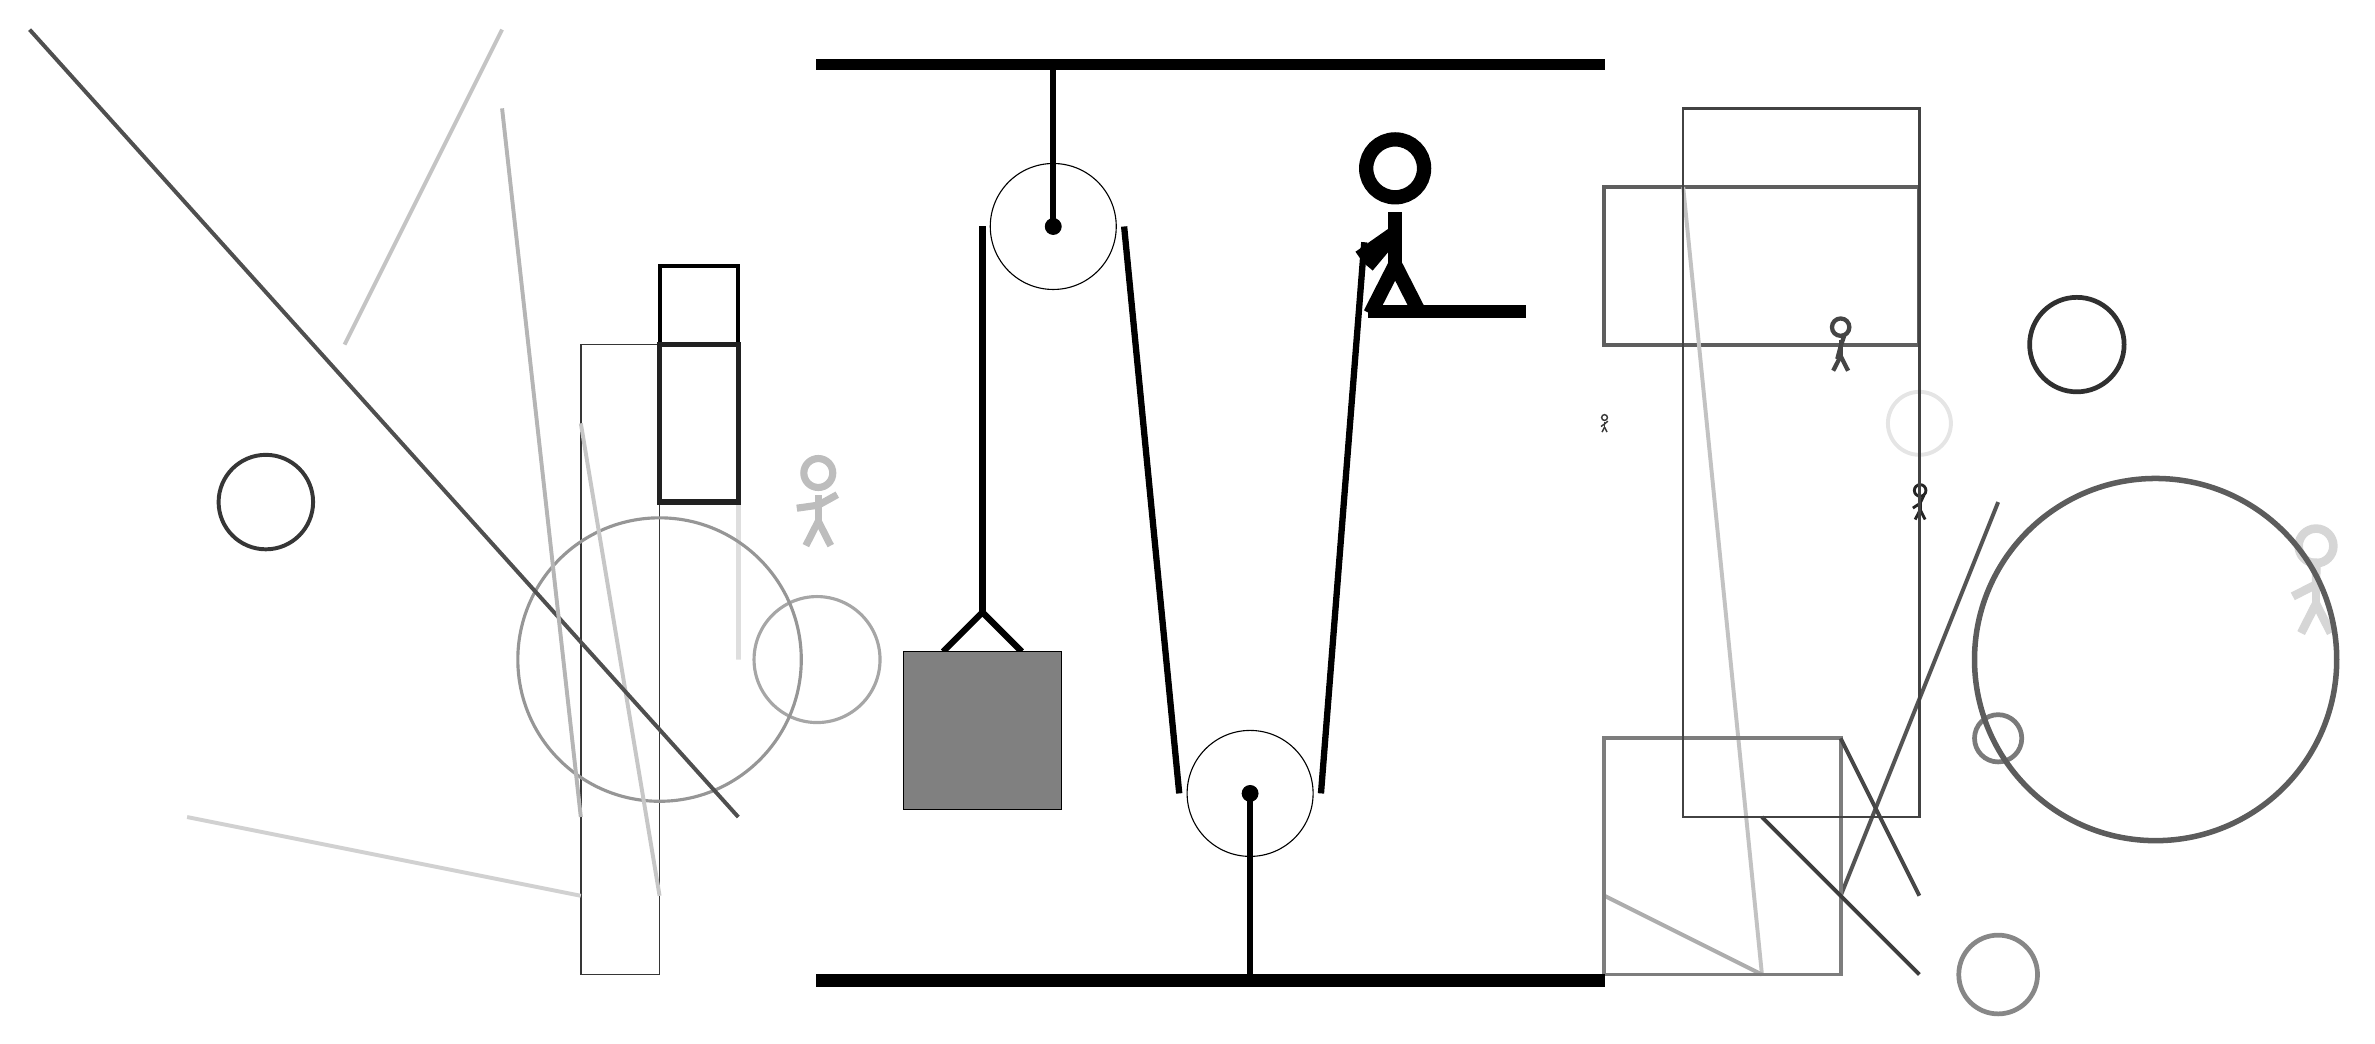
\begin{tikzpicture}
			%%%%% START %%%%%
			
			\draw[fill=black] (-2, 11.5) rectangle (8, 11.625);
			
			\draw (3.5, 2.3) circle (0.8);
			\draw[fill=black] (3.5, 2.3) circle (0.1);
			\draw[line width=0.8mm] (3.5, 2.3) -- (3.5, 0);
			
			\draw[line width=0.7mm, color=black!13] (-3, 8) rectangle (-3, 4);
			
			\draw[line width=0.2mm, color=black!79] (-4, 8) rectangle (-5, 0);
			\draw[line width=0.5mm, color=black!63] (8, 8) rectangle (12, 10);
			\draw [line width=0.4mm, color=black!35](-2, 4) circle (0.8);
			
			\draw [line width=0.6mm, color=black!81](14, 8) circle (0.6);
			\draw[line width=0.5mm, color=black!24](10, 0) -- (9, 10);
			
			\node[line width=0.6mm, color=black!16] at (17, 5) {\Strichmaxerl[6][27][89]};
			\draw[line width=0.5mm, color=black!67](13, 6) -- (11, 1);
			\draw [line width=0.6mm, color=black!52](13, 3) circle (0.3);
			
			\draw [line width=0.5mm, color=black!10](12, 7) circle (0.4);
			\node[line width=0.4mm, color=black!86] at (12, 6) {\Strichmaxerl[2][33][65]};
			\draw [line width=0.7mm, color=black!64](15, 4) circle (2.3);
			\draw[line width=0.5mm, color=black!32](10, 0) -- (8, 1);
			\draw[line width=0.5mm, color=black!100] (-3, 9) rectangle (-4, 6);
			\node[line width=0.2mm, color=black!73] at (11, 8) {\Strichmaxerl[3][75][72]};
			\draw[line width=0.5mm, color=black!51] (8, 3) rectangle (11, 0);
			
			\draw [line width=0.6mm, color=black!47](13, 0) circle (0.5);
			\node[line width=0.3mm, color=black!78] at (8, 7) {\Strichmaxerl[1][36][40]};
			\draw [line width=0.5mm, color=black!79](-9, 6) circle (0.6);
			\draw [line width=0.4mm, color=black!41](-4, 4) circle (1.8);
			\draw[line width=0.5mm, color=black!76](12, 0) -- (10, 2);
			\node[line width=0.7mm, color=black!26] at (-2, 6) {\Strichmaxerl[5][8][29]};
			
			\draw[line width=0.5mm, color=black!22](-4, 1) -- (-5, 7);
			\draw[line width=0.5mm, color=black!72](11, 3) -- (12, 1);
			\draw[line width=0.3mm, color=black!74] (9, 2) rectangle (12, 11);
			
			\draw[line width=0.5mm, color=black!69](-3, 2) -- (-12, 12);
			\draw[line width=0.5mm, color=black!23](-6, 12) -- (-8, 8);
			\draw[line width=0.5mm, color=black!18](-5, 1) -- (-10, 2);
			\draw[line width=0.5mm, color=black!29](-5, 2) -- (-6, 11);
			
			\draw[line width=0.7mm, color=black!87] (-4, 8) rectangle (-3, 6);
			
			\draw (1, 9.5) circle (0.8);
			\draw[fill=black] (1, 9.5) circle (0.1);
			\draw[line width=0.8mm] (1, 11.5) -- (1, 9.5);
			
			\draw[line width=0.8mm](-0.4, 4.1) --  (0.1, 4.6) -- (0.6, 4.1);
			\draw[fill=black!50] (-0.9, 4.1) rectangle (1.1, 2.1);
			
			\draw[line width=0.8mm](0.1, 9.5) -- (0.1, 4.6);
			\centerarc[line width=0.8mm](1, 9.5)(180:0:0.9)
			\draw[line width=0.8mm](1.9, 9.5) -- (2.6, 2.3);
			\centerarc[line width=0.8mm](3.5, 2.3)(180:360:0.9)
			\draw[line width=0.8mm](4.4, 2.3) -- (4.95, 9.3);
			
			\node at (5.3, 9.5) {\Strichmaxerl[10][35][-130]};
			\draw[fill=black] (5, 8.5) rectangle (7, 8.35);
			
			\draw[fill=black] (-2, 0) rectangle (8, -0.15);
			
			%%%%% END %%%%%
		\end{tikzpicture}
	\end{figure}	
\end{document}